\documentclass{article}

\usepackage{fancyhdr}
\usepackage{ragged2e}
\usepackage{graphicx}
\usepackage{caption}
\usepackage{geometry}
\usepackage{amsmath}
\usepackage{rotating}

\usepackage{listings}
\usepackage{color}

\definecolor{dkgreen}{rgb}{0,0.6,0}
\definecolor{gray}{rgb}{0.5,0.5,0.5}
\definecolor{mauve}{rgb}{0.58,0,0.82}

\lstset{frame=tb,
  language=Java,
  aboveskip=3mm,
  belowskip=3mm,
  showstringspaces=false,
  columns=flexible,
  basicstyle={\small\ttfamily},
  numbers=none,
  numberstyle=\tiny\color{gray},
  keywordstyle=\color{blue},
  commentstyle=\color{dkgreen},
  stringstyle=\color{mauve},
  breaklines=true,
  breakatwhitespace=true,
  tabsize=4
}

\setcounter{secnumdepth}{1}

\usepackage{chngcntr}
\counterwithin{figure}{section}

\renewcommand*{\thepage}{C\arabic{page}}

\pagestyle{fancy}
\lhead{ACME Robotics}
\chead{\#8367}
\rhead{\ifcontents Contents \else Week \thesection \fi}

\newif\ifcontents
\contentstrue

\makeatletter
\renewcommand{\@seccntformat}[1]{}
\makeatother

\begin{document}\contentsfalse

\subsection{Assembling Rev Linear Motion Slides for the Rake}
%! Assembling and Attaching the Linear slides and Rake system.
Continuing the manufacturing process, Jon and Aidan assembled the linear slides for the intake rake. The team wanted to create a four stage slide so that no matter where the robot was around the crater it could reach every cube or ball in the crater. However the team had only bought two linear slide kits which would only allow for a two stage slide. John and Aidan found extra parts from the previous years linear slide system. This allowed for there to be a three stage system which would give them enough length to reach to almost the back of the crater and get plenty of minerals. After constructing the slides, Jon and Aidan had to fine tune them to get them both to run smoothly and with little resistance because there was only going to be one motor powering both slides and if there was too much resistance the motor wouldn't be able to power them. After these were constructed, Aidan went on to build the rake portion of the slide and Jon attached the slides to the robot. Jon did this by using Tetrix L brackets and screwing them into the outside plate of the drive train. This made sure the slides were inside the 18 inches and were firmly attached to the robot in case they got bumped by another robot during competition. To create the rake Aidan needed to find a way to minimize the length it added to the robot. The rake had to sit low enough so that it could tuck under the intake system but it needed to be high enough so that it would pass over the crater wall. Aidan solved this by having the axle of the rake sit exactly 4 inches above the ground.

\begin{figure}
    \centering
    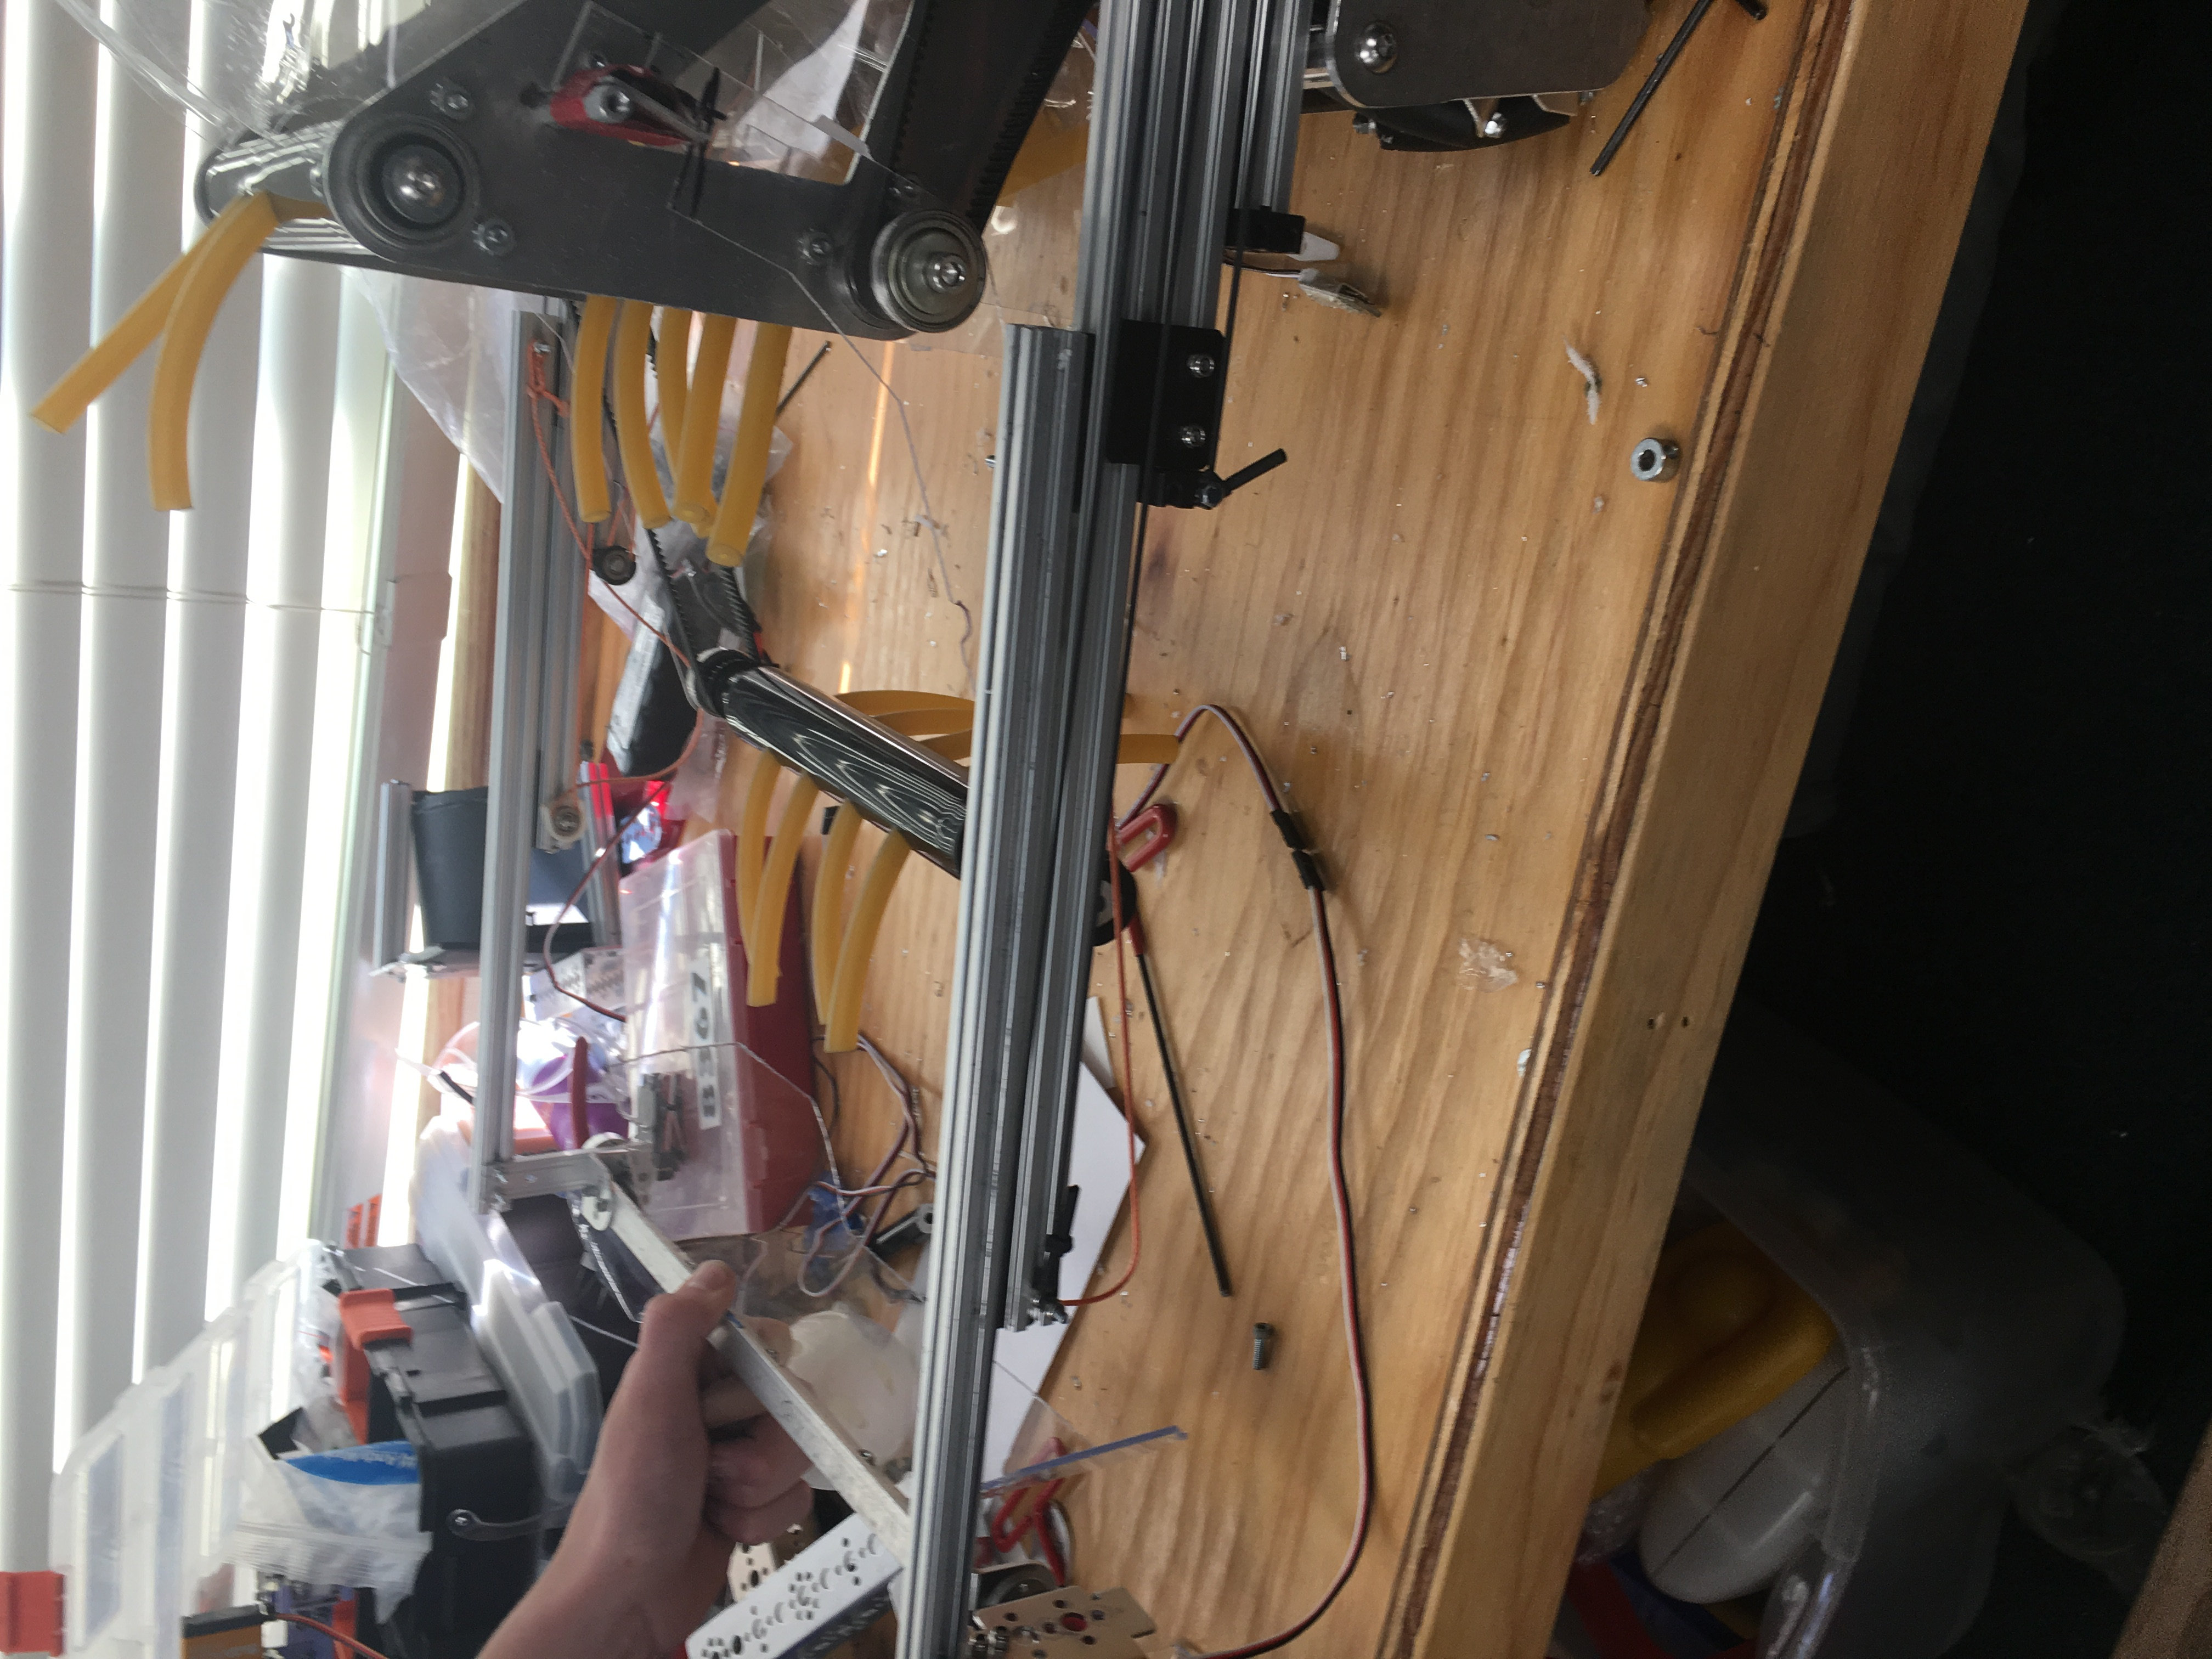
\includegraphics[width=.6 \textwidth, angle=-90 ]{11_11-12/images/rake_slides.JPG}
    \caption{Rake and Slides}
    \label{fig:Intake CAD}
\end{figure}

\subsection{Shield Attachment}
%!Attaching the Shield to the robot.
After the shield was built it needed to be attached to the robot. The attachment piece would attach to the side plates of the intake But couldn't attach to the back of the sorter because the screws on the attachment might catch cubes when the went up the intake. To solve this Aidan created brackets that would allow the attachment piece to screw into the shield on the sides which would decrease the likely-hood of cubes getting caught.

\begin{figure}
    \centering
    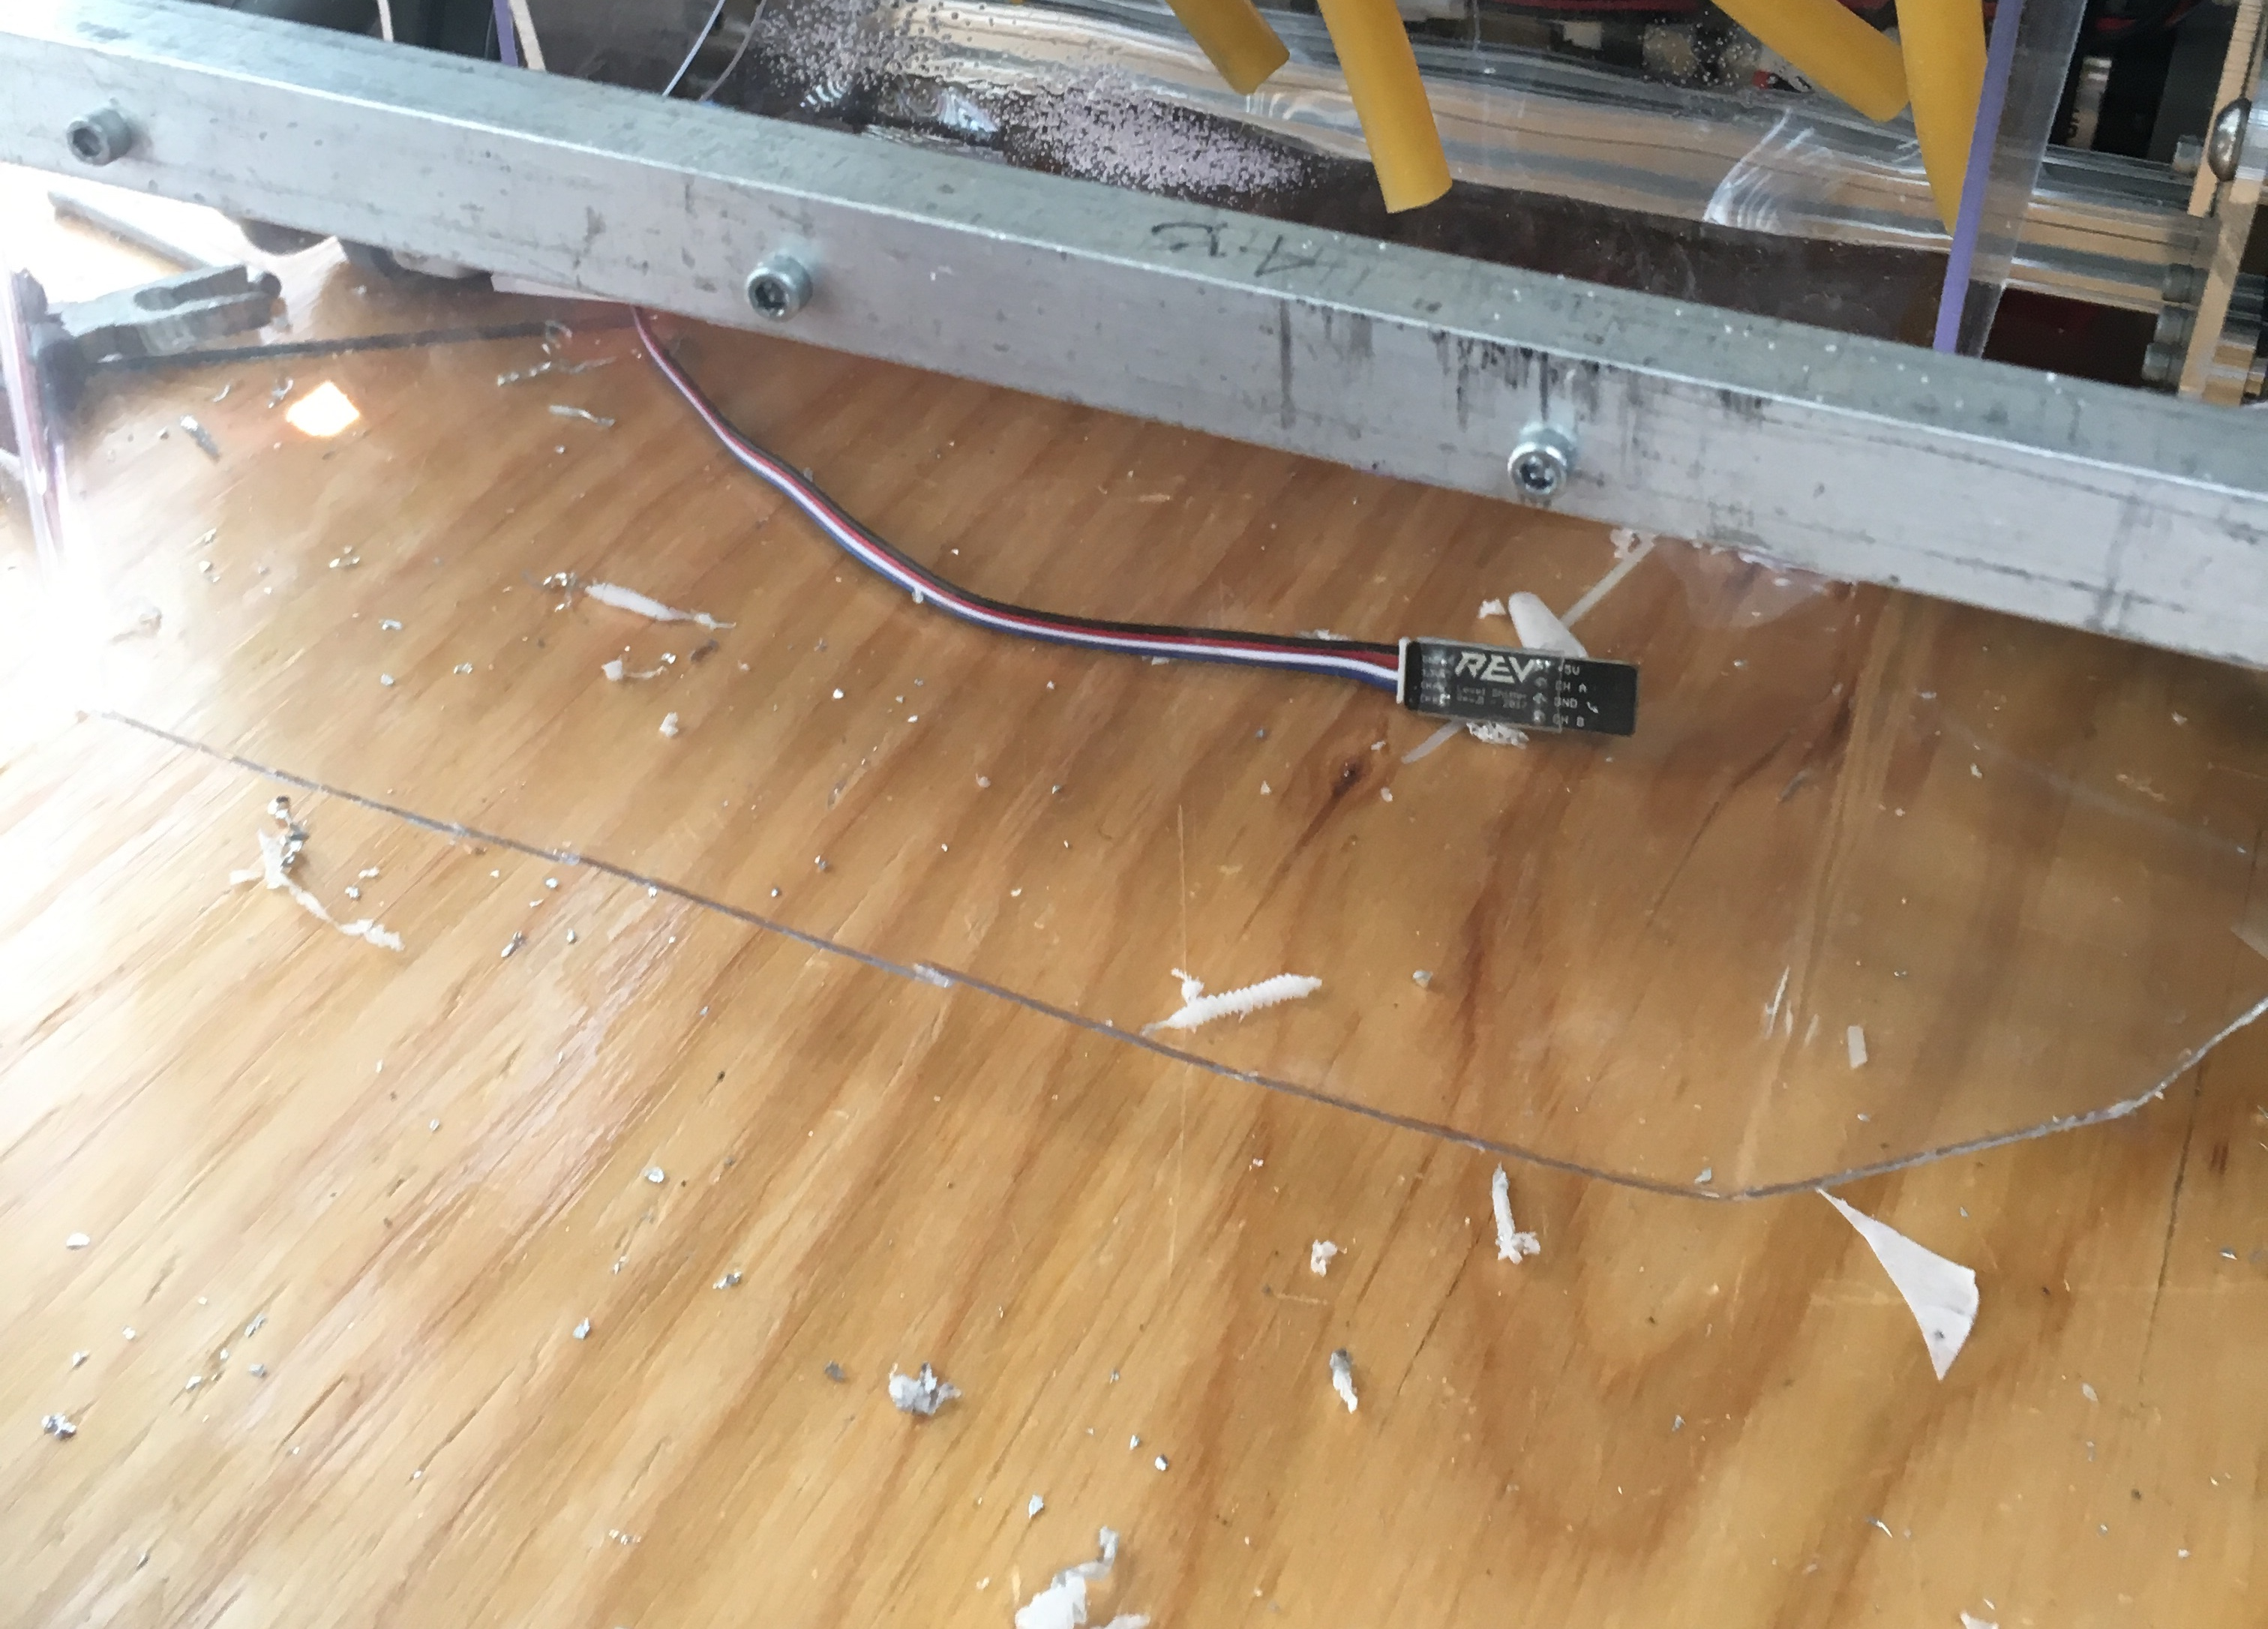
\includegraphics[width=.6 \textwidth]{11_11-12/images/rake.jpg}
    \caption{Rake Shield}
    \label{fig:rakeshield}
\end{figure}
\end{document}